\documentclass{standalone}

\usepackage{tikz}
\usepackage{circuitikz}

\tikzset{block/.style = {draw, fill=white, very thick, rectangle, minimum height=1cm, minimum width=2cm},
         lblock/.style={draw,fill=white,very thick, rectangle, minimum height=3cm, minimum width=1cm},
         sum/.style= {draw, fill=white, very thick, circle, node distance=0.5cm}}

         
\begin{document}
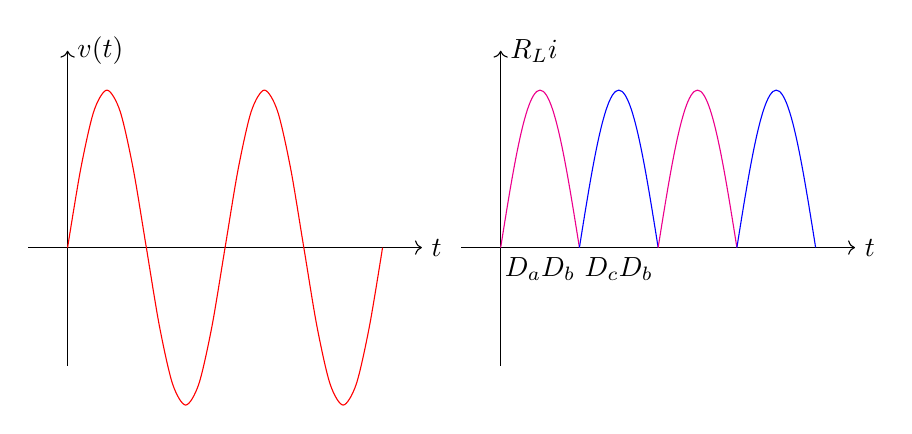
\begin{tikzpicture}[scale=2]
    \draw[->](-0.25,0)--(2.25,0)node[right]{$t$};
    \draw[->](0,-0.75)--(0,1.25)node[right]{$v(t)$};

    \draw[red,smooth, domain=0:2]plot (\x,{sin(2*pi*\x r)});

    \draw[->](2.5,0)--(5,0)node[right]{$t$};
    \draw[->](2.75,-0.75)--(2.75,1.25)node[right]{$R_Li$};
    \draw[magenta,smooth, domain=2.75:3.25]plot (\x,{sin(2*pi*(\x-2.75) r)});    
    \draw[blue,smooth, domain=3.25:3.75]plot (\x,{sin(2*pi*(\x-3.25) r)});
    \draw[magenta,smooth, domain=3.75:4.25]plot (\x,{sin(2*pi*(\x-2.75) r)});
    \draw[blue,smooth, domain=4.25:4.75]plot (\x,{sin(2*pi*(\x-3.25) r)});
    \node[below] at(3,0){$D_aD_b$};
    \node[below] at(3.5,0){$D_cD_b$};
\end{tikzpicture}
\end{document}